\begin{figure}[ht]
		\centering
		\resizebox{0.75\textwidth}{!}{%
			\begin{tikzpicture}[>=stealth, line width=0.8pt, font=\small,
				nodo/.style  = {circle, fill=white, draw=black,
					inner sep=0pt, minimum size=5pt, line width=0.8pt},
				]
				
				%% ── Parametri geometrici globali ─────────────────────────────────
				\def\L{3.0}      % luce ell
				\def\tw{0.20}    \def\thA{0.34}  \def\thR{0.28}
				\def\sr{0.07}    \def\bw{0.14}   \def\gw{0.26}
				\def\GapP{2.5}   % gap orizzontale tra i due pannelli
				
				%% Posizioni nodi
				\pgfmathsetmacro{\xB}{\L}
				\pgfmathsetmacro{\xG}{0.5*\L}
				\pgfmathsetmacro{\XPb}{\L + \GapP}
				
				%% =================================================================
				%% PANNELLO (a) — SISTEMA REALE: trave appoggiata con carico F in G
				%% =================================================================
				\begin{scope}[xshift=0cm, yshift=0cm]
					
					%% Trave
					\draw[line width=2.2pt] (0,0) -- (\xB,0);
					
					%% Etichette nodi
					\node[above=0.04] at (0,0)   {$A$};
					\node[below=0.04] at (\xG,0) {$G$};
					\node[above=0.04] at (\xB,0) {$B$};
					
					%% Cerniera in A
					\draw (0,0) -- ++(-\tw,-\thA) -- ++(2*\tw,0) -- cycle;
					\draw (-\gw,-\thA) -- (\gw,-\thA);
					\foreach \x in {-0.20,-0.10,0,0.10,0.20}
					\draw[thin] (\x,-\thA) -- ++(-.07,-.09);
					\node[nodo] at (0,0) {};
					
					%% Carrello verticale in B
					\draw (\xB,0) -- ++(-\tw,-\thR) -- ++(2*\tw,0) -- cycle;
					\draw (\xB-\gw,-\thR) -- (\xB+\gw,-\thR);
					\draw (\xB-\bw,-\thR-0.10) circle (2pt);
					\draw (\xB+\bw,-\thR-0.10) circle (2pt);
					\draw (\xB-\gw,-\thR-0.20) -- (\xB+\gw,-\thR-0.20);
					\foreach \x in {-0.20,-0.10,0,0.10,0.20}
					\draw[thin] (\xB+\x,-\thR-0.20) -- ++(-.07,-.09);
					\node[nodo] at (\xB,0) {};
					
					%% Carico F verticale verso il basso in G
					\def\Fh{0.85}
					\draw[->, line width=1.0pt] (\xG, \Fh) -- (\xG, 0.05);
					\node[right=0.05, font=\small] at (\xG, 0.5*\Fh) {$F$};
					
					%% Etichetta pannello
					\node[font=\small, below=0.05] at (0.5*\xB, -1.10)
					{(a) Sistema reale};
					
				\end{scope}
				
				%% =================================================================
				%% PANNELLO (b) — PROBLEMA VIRTUALE: cedimento unitario in A
				%% =================================================================
				\begin{scope}[xshift=\XPb cm, yshift=0cm]
					
					%% Spostamento verticale del cedimento (unità grafica)
					\def\sa{0.55}
					
					%% Trave indeformata (riferimento, in tratteggio grigio)
					\draw[line width=0.6pt, gray] (0,0) -- (\xB,0);
					
					%% Trave virtuale (configurazione deformata, ruotata attorno a B)
					%% A scende di sa, B resta fermo, G scende di sa/2
					\draw[line width=2.2pt] (0,-\sa) -- (\xB,0);
					
					%% Etichette nodi (sulla trave virtuale)
					\node[above=0.04] at (0,0)        {$A$};
					\node[above=0.04] at (\xG,0)  {$G$};
					\node[above=0.04] at (\xB,0)         {$B$};
					
					%% Carrello in B (resta come nel reale)
					\draw (\xB,0) -- ++(-\tw,-\thR) -- ++(2*\tw,0) -- cycle;
					\draw (\xB-\gw,-\thR) -- (\xB+\gw,-\thR);
					\draw (\xB-\bw,-\thR-0.10) circle (2pt);
					\draw (\xB+\bw,-\thR-0.10) circle (2pt);
					\draw (\xB-\gw,-\thR-0.20) -- (\xB+\gw,-\thR-0.20);
					\foreach \x in {-0.20,-0.10,0,0.10,0.20}
					\draw[thin] (\xB+\x,-\thR-0.20) -- ++(-.07,-.09);
					\node[nodo] at (\xB,0) {};
					
					%% Cerniera in A rimossa: indico con cerchietto bianco la
					%% libertà di traslazione verticale
					\node[nodo] at (0,-\sa) {};
					
					%% Cedimento s*_A: doppia freccia verticale con quota
					\draw[->, line width=0.6pt, gray]
					(-0.40, 0) -- (-0.40, -\sa);
					\node[font=\footnotesize, left, color=black!60]
					at (-0.45, -0.5*\sa) {$s^*_A = 1$};
					
					%% Spostamento v*_G: doppia freccia verticale, lunghezza sa/2
					\draw[->, line width=0.6pt, gray]
					(\xG-0.30, 0) -- (\xG-0.30, -0.5*\sa);
					\node[font=\footnotesize, left, color=black!60]
					at (\xG-0.35, -0.27*\sa) {$v^*_G = \tfrac{1}{2}$};
					
					%% Etichetta pannello
					\node[font=\small, below=0.05] at (0.5*\xB, -1.10)
					{(b) Problema virtuale};
					
				\end{scope}
				
			\end{tikzpicture}%
		}
		\caption{TSV per il calcolo della reazione $R_A$ in una trave
			semplicemente appoggiata sotto carico $F$ in mezzeria.}
		\label{fig:TSV_trave_semplice}
	\end{figure}
